% =============================================================================
\chapter{Weather and Climate of India}
\label{ch:climate}
% =============================================================================
This chapter gives the climate background needed for the rest of this guide: how weather differs across the
regions of India, which factors cause these differences, and where Himachal Pradesh fits.

\section{Weather Regions of India}
India stretches over about 30 degrees of latitude, from the equatorial south to the high Himalaya, so its weather
varies strongly from region to region. Two common ways of dividing it are used here.

\textbf{IMD homogeneous regions.} For monsoon monitoring and forecasting, IMD groups its meteorological subdivisions
into four broad regions with similar rainfall: Northwest India, Central India, South Peninsula, and East \& Northeast
India (Figure~\ref{fig:indiaregions}). Their normal June--September rainfall ranges from 587.6\,mm in Northwest India
to 1{,}367.3\,mm in East \& Northeast India. Himachal Pradesh belongs to \textbf{Northwest
India}, the driest of the four in the monsoon and the one most affected by winter western disturbances and pre-monsoon
heat.

\begin{figure}[H]
\centering
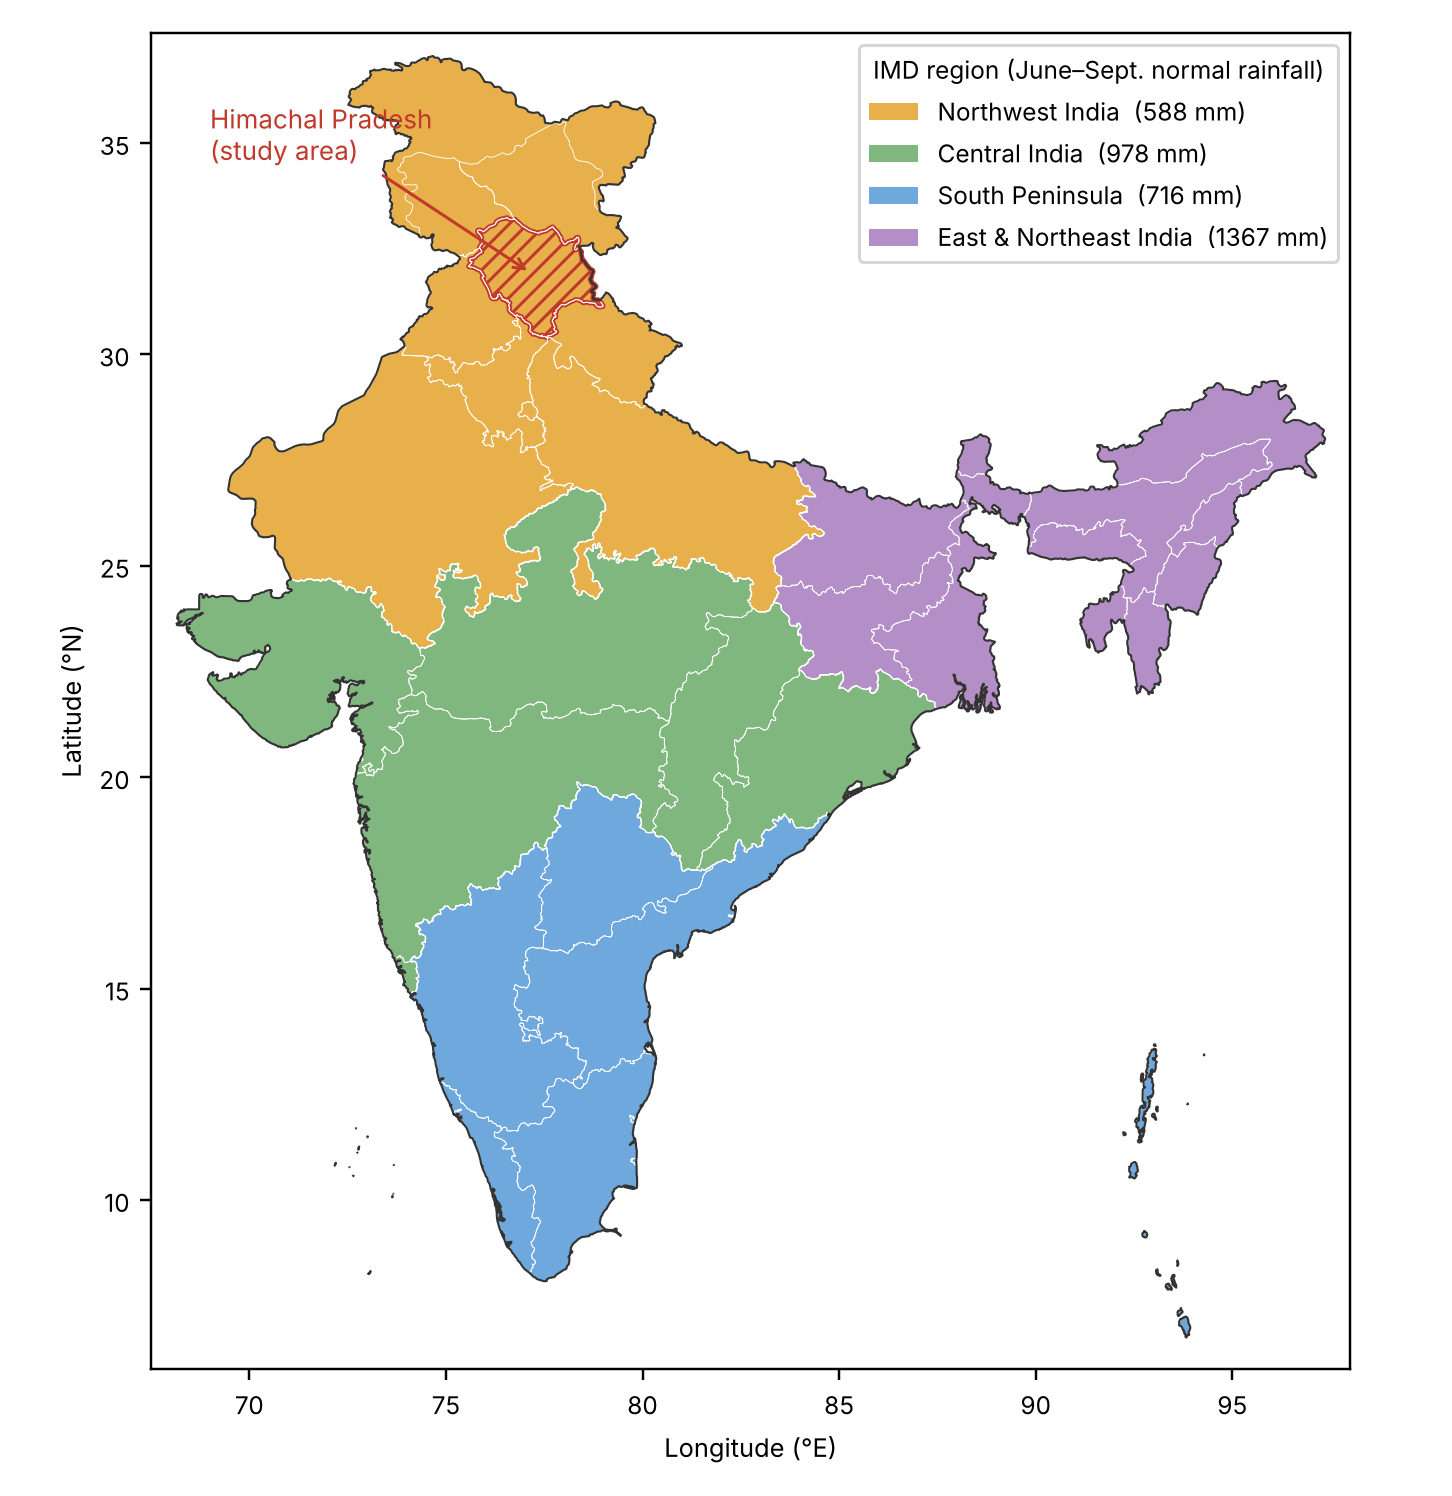
\includegraphics[width=0.74\textwidth]{fig_india_regions.png}
\caption{IMD's four homogeneous rainfall regions, drawn here by state, with their normal June--September rainfall
(1971--2020). IMD defines the regions by meteorological subdivision, so the state outlines are
an approximation. Himachal Pradesh, the study area, is hatched. Boundaries: Natural Earth (India's official view).}
\label{fig:indiaregions}
\end{figure}

\textbf{Climate types.} By temperature and rainfall, the country also falls into a few broad climate types
(Figure~\ref{fig:indiaclimate} and Table~\ref{tab:climtypes}).

\begin{figure}[H]
\centering
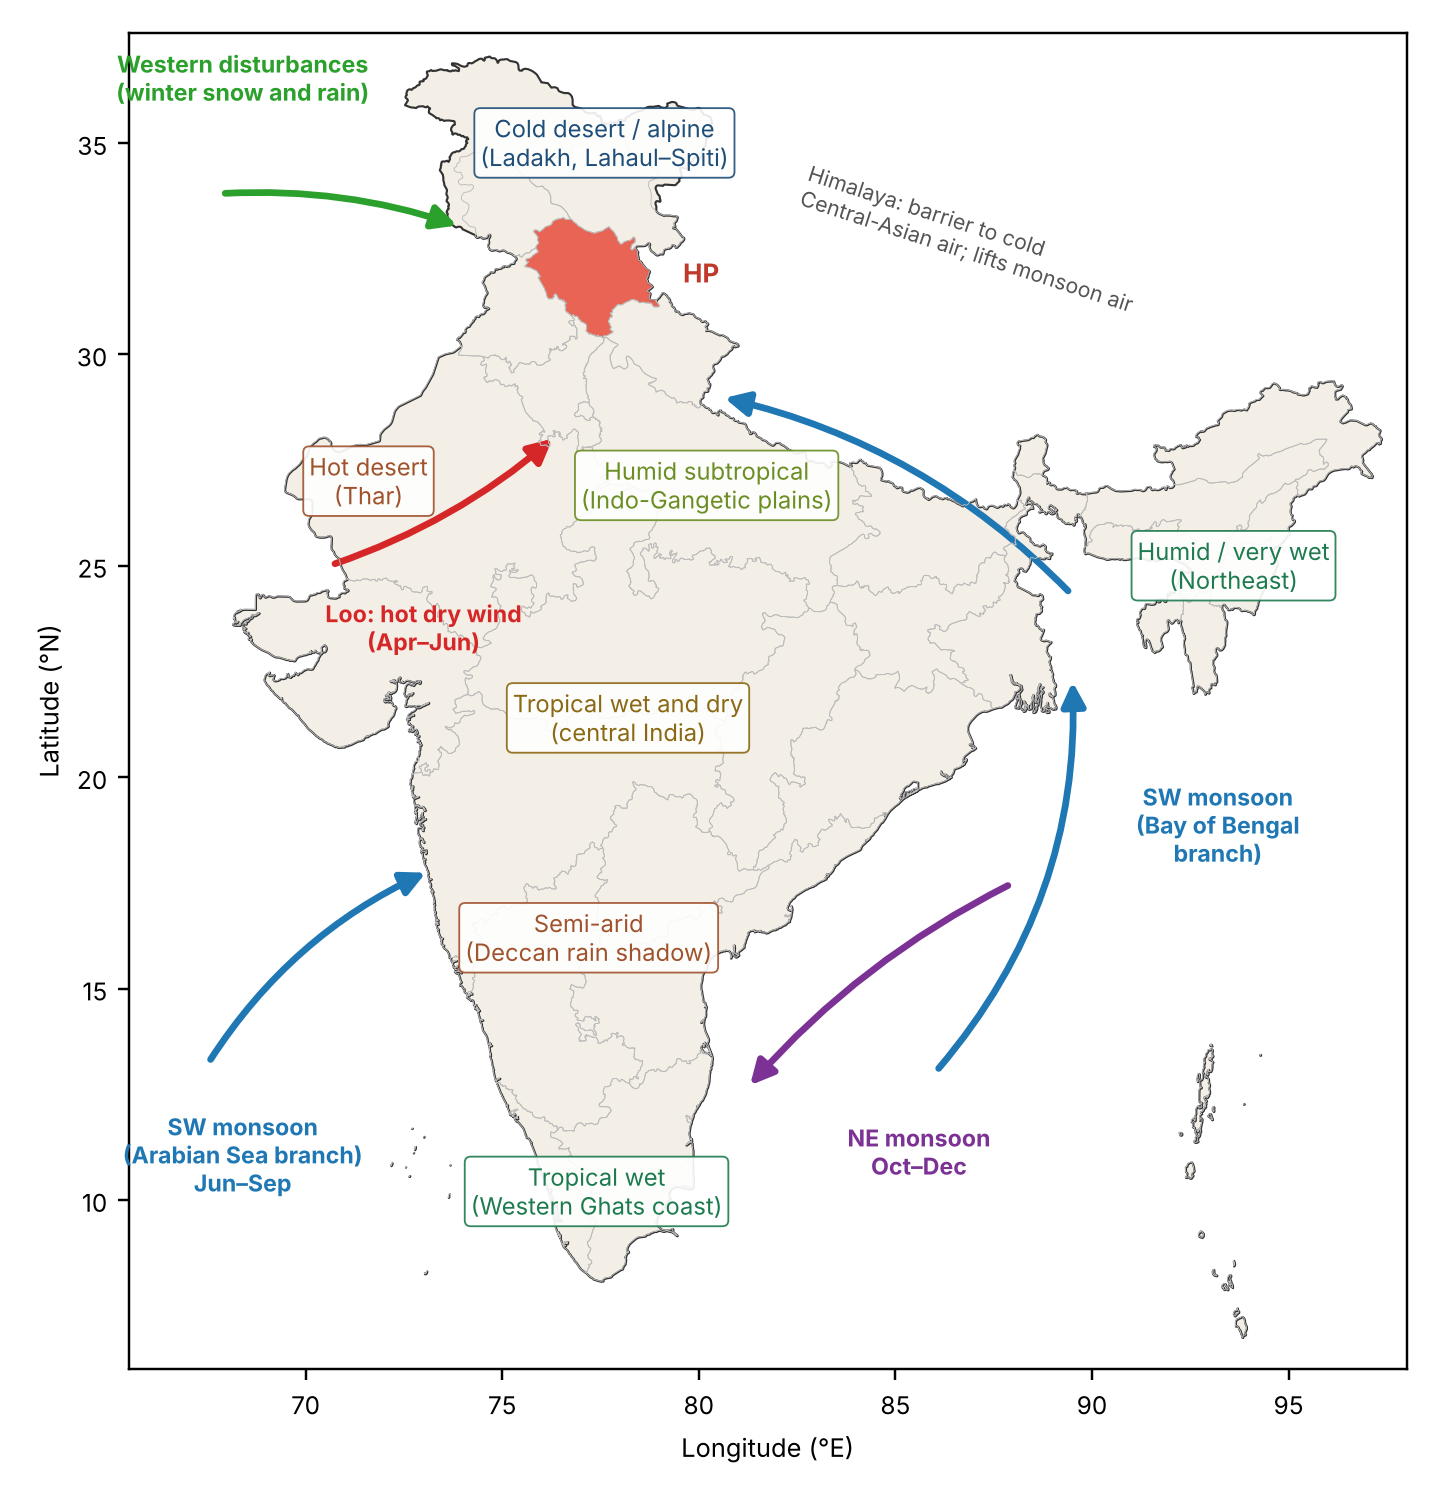
\includegraphics[width=0.74\textwidth]{fig_india_climate.png}
\caption{Broad climate types of India (labels placed at their typical location; no exact borders are implied) and
the main winds that shape them. Blue: the two branches of the southwest monsoon; purple: the northeast monsoon; green:
western disturbances; red: the hot \emph{loo} wind. Himachal Pradesh is shown in red.}
\label{fig:indiaclimate}
\end{figure}

\begin{table}[H]\footnotesize
\centering
\caption{Broad climate types of India.}
\label{tab:climtypes}
\begin{tabular}{|p{3.2cm}|p{4.2cm}|p{7.0cm}|}
\hline
\textbf{Climate type} & \textbf{Where} & \textbf{Main features}\\ \hline
Tropical wet & Western Ghats coast (Kerala, Konkan), parts of the Northeast & Hot and humid all year; very heavy
monsoon rain on slopes facing the wind.\\ \hline
Tropical wet and dry & Most of central and peninsular India & Hot summers, a clear wet season (monsoon) and a long dry
season.\\ \hline
Semi-arid & Interior Deccan (in the rain shadow of the Western Ghats), parts of Gujarat and Rajasthan & Low, unreliable
rain; hot summers.\\ \hline
Hot desert & Thar desert (western Rajasthan) & Very little rain; very hot days and cool nights; dust storms.\\ \hline
Humid subtropical & Indo-Gangetic plains, Himalayan foothills (including lower Himachal Pradesh) & Hot summers with
heatwaves, wet monsoon, cool to cold winters with fog.\\ \hline
Mountain (temperate to alpine) & Himalaya (middle and high Himachal Pradesh, Uttarakhand, Jammu \& Kashmir, Sikkim)
& Temperature falls with height; winter snow; climate changes over short distances.\\ \hline
Cold desert & Ladakh, Lahaul--Spiti and upper Kinnaur & Behind the main Himalayan ranges; very dry, very cold
winters, strong sunshine.\\ \hline
\end{tabular}
\end{table}

\section{Factors that Affect Weather in India}
The regional differences above come from a small set of physical factors (Figure~\ref{fig:factors}).

\begin{figure}[H]
\centering
\begin{tikzpicture}[
  fac/.style={draw=blue!55!black,fill=blue!6,rounded corners=2pt,text width=3.4cm,align=center,font=\footnotesize,minimum height=1.25cm,inner sep=3pt},
  mid/.style={draw=orange!70!black,fill=orange!12,rounded corners=3pt,text width=3.0cm,align=center,font=\small\bfseries,minimum height=1.4cm},
  ar2/.style={-{Stealth[length=2mm]},thick,black!55}]
\node[mid] (c) at (0,0) {Weather and climate of a place};
\node[fac] (f1) at (-5.0, 2.6) {\textbf{Latitude}\\ how high the sun is and how long the day};
\node[fac] (f2) at (0, 2.9) {\textbf{Altitude}\\ about 6.5\,$^\circ$C cooler per km of height};
\node[fac] (f3) at (5.0, 2.6) {\textbf{Himalaya as a barrier}\\ blocks cold Central-Asian air, traps monsoon air};
\node[fac] (f4) at (-5.4, 0) {\textbf{Distance from the sea}\\ coasts mild and humid; interior has larger swings};
\node[fac] (f5) at (5.4, 0) {\textbf{Relief and slope}\\ wet windward slopes, dry rain shadows, valley heat};
\node[fac] (f6) at (-5.0,-2.6) {\textbf{Monsoon winds}\\ seasonal reversal of winds brings the summer rain};
\node[fac] (f7) at (0,-2.9) {\textbf{Western disturbances and jet stream}\\ winter storms from the west};
\node[fac] (f8) at (5.0,-2.6) {\textbf{Land surface and ocean state}\\ dry soil heats faster; El Ni\~no and the Indian Ocean Dipole};
\foreach \f in {f1,f2,f3,f4,f5,f6,f7,f8} \draw[ar2] (\f) -- (c);
\end{tikzpicture}
\caption{The main factors that control the weather and climate of a place in India.}
\label{fig:factors}
\end{figure}

\begin{enumerate}
\item \textbf{Latitude.} The Tropic of Cancer crosses the middle of India. The south is close to the equator and warm
all year; the north has a large difference between summer and winter.
\item \textbf{Altitude.} Air cools by about 6.5\,$^\circ$C for each kilometre of height on average. This is why the
same calendar day can be 40\,$^\circ$C in the plains and below freezing in the high Himalaya, and why this project
sets a separate threshold for every grid cell (Chapter~\ref{ch:extreme}).
\item \textbf{The Himalaya as a barrier.} The mountain wall keeps the cold, dry winter air of Central Asia out of
northern India, and in summer forces the moist monsoon winds to rise and release their rain on the southern slopes.
\item \textbf{Distance from the sea.} The sea warms and cools slowly, so coastal places have small daily and yearly
temperature ranges and high humidity. Inland places, far from the sea, have hotter summers and colder winters.
\item \textbf{Relief and slope (orographic effect).} When moist air is pushed up a mountain it cools, its water
vapour condenses and rain falls on the windward side; the air that comes down the other side is dry and warm, leaving
a \emph{rain shadow} (Figure~\ref{fig:orographic}). The Western Ghats and the Deccan, and the main Himalayan ranges
and Lahaul--Spiti, are two such pairs.
\item \textbf{Monsoon winds.} In summer the land heats much faster than the Indian Ocean; low pressure over north-west
India draws in moist south-westerly winds from the sea (the \emph{southwest monsoon}, with an Arabian Sea branch and a
Bay of Bengal branch). In winter the winds reverse and blow from the land (the \emph{northeast monsoon}), giving rain
only where they cross the Bay of Bengal, mainly in Tamil Nadu.
\item \textbf{Western disturbances and the jet stream.} In winter and spring, storms that form over the Mediterranean
region travel east along the subtropical westerly jet stream and bring snow and rain to the western Himalaya. They are
the main source of winter precipitation in Himachal Pradesh.
\item \textbf{Land surface and ocean state.} Dry soil uses less of the sun's energy for evaporation, so more of it
heats the air: dry spells before or during the summer make heat extremes more likely. On a larger scale, El Ni\~no
events in the Pacific and the Indian Ocean Dipole change the strength of the monsoon from year to year.
\end{enumerate}

\begin{figure}[H]
\centering
\begin{tikzpicture}[x=1cm,y=1cm]
\fill[brown!35] (0,0) -- (3.5,0) .. controls (5,1.5) and (5.6,3.1) .. (6.3,3.4) .. controls (7,3.1) and (7.6,1.5) .. (9.1,0) -- (12.6,0) -- (12.6,-0.3) -- (0,-0.3) -- cycle;
\draw[brown!60!black,thick] (0,0) -- (3.5,0) .. controls (5,1.5) and (5.6,3.1) .. (6.3,3.4) .. controls (7,3.1) and (7.6,1.5) .. (9.1,0) -- (12.6,0);
\draw[-{Stealth[length=3mm]},very thick,blue!70!black] (0.2,0.7) -- (3.3,0.7) .. controls (4.6,1.4) and (5.3,3.4) .. (6.3,4.0);
\draw[-{Stealth[length=3mm]},very thick,red!70!black] (6.3,4.0) .. controls (7.4,3.4) and (8.1,1.6) .. (9.4,0.9) -- (12.3,0.9);
\foreach \x in {4.1,4.7,5.3} \draw[fill=gray!25,draw=gray!60] (\x,3.6) ellipse (0.55 and 0.32);
\foreach \x in {3.9,4.2,4.5,4.8,5.1,5.4} \draw[blue!60,thick] (\x,3.2) -- (\x-0.12,2.2);
\node[font=\footnotesize,align=center,blue!60!black] at (1.8,1.5) {moist air from the sea};
\node[font=\footnotesize,align=center] at (4.0,4.45) {air rises, cools:\\clouds and rain};
\node[font=\footnotesize,align=center] at (2.6,-0.75) {\textbf{windward side}: wet};
\node[font=\footnotesize,align=center,red!60!black] at (10.6,1.7) {dry, warm descending air};
\node[font=\footnotesize,align=center] at (10.6,-0.75) {\textbf{rain shadow}: dry};
\end{tikzpicture}
\caption{The orographic effect: mountains make one side wet and the other dry.}
\label{fig:orographic}
\end{figure}

\section{Himachal Pradesh}
Himachal Pradesh lies in Northwest India on the southern side of the western Himalaya. Its height rises from about
300\,m near Una in the south-west to above 6{,}000\,m in the north-east, so it holds several climates within a short
distance. Using the elevation bands of the state's agro-climatic zones, the 529 grid cells of this project fall into
four groups (Figure~\ref{fig:hpzones}): 95 sub-tropical low-hill cells (below 1{,}000\,m), 47 sub-temperate mid-hill
cells (1{,}000--1{,}500\,m), 89 wet temperate high-hill cells (1{,}500--2{,}500\,m) and 298 dry temperate or cold-desert
cells (above 2{,}500\,m). More than half of the state therefore lies above 2{,}500\,m.

\begin{figure}[H]
\centering
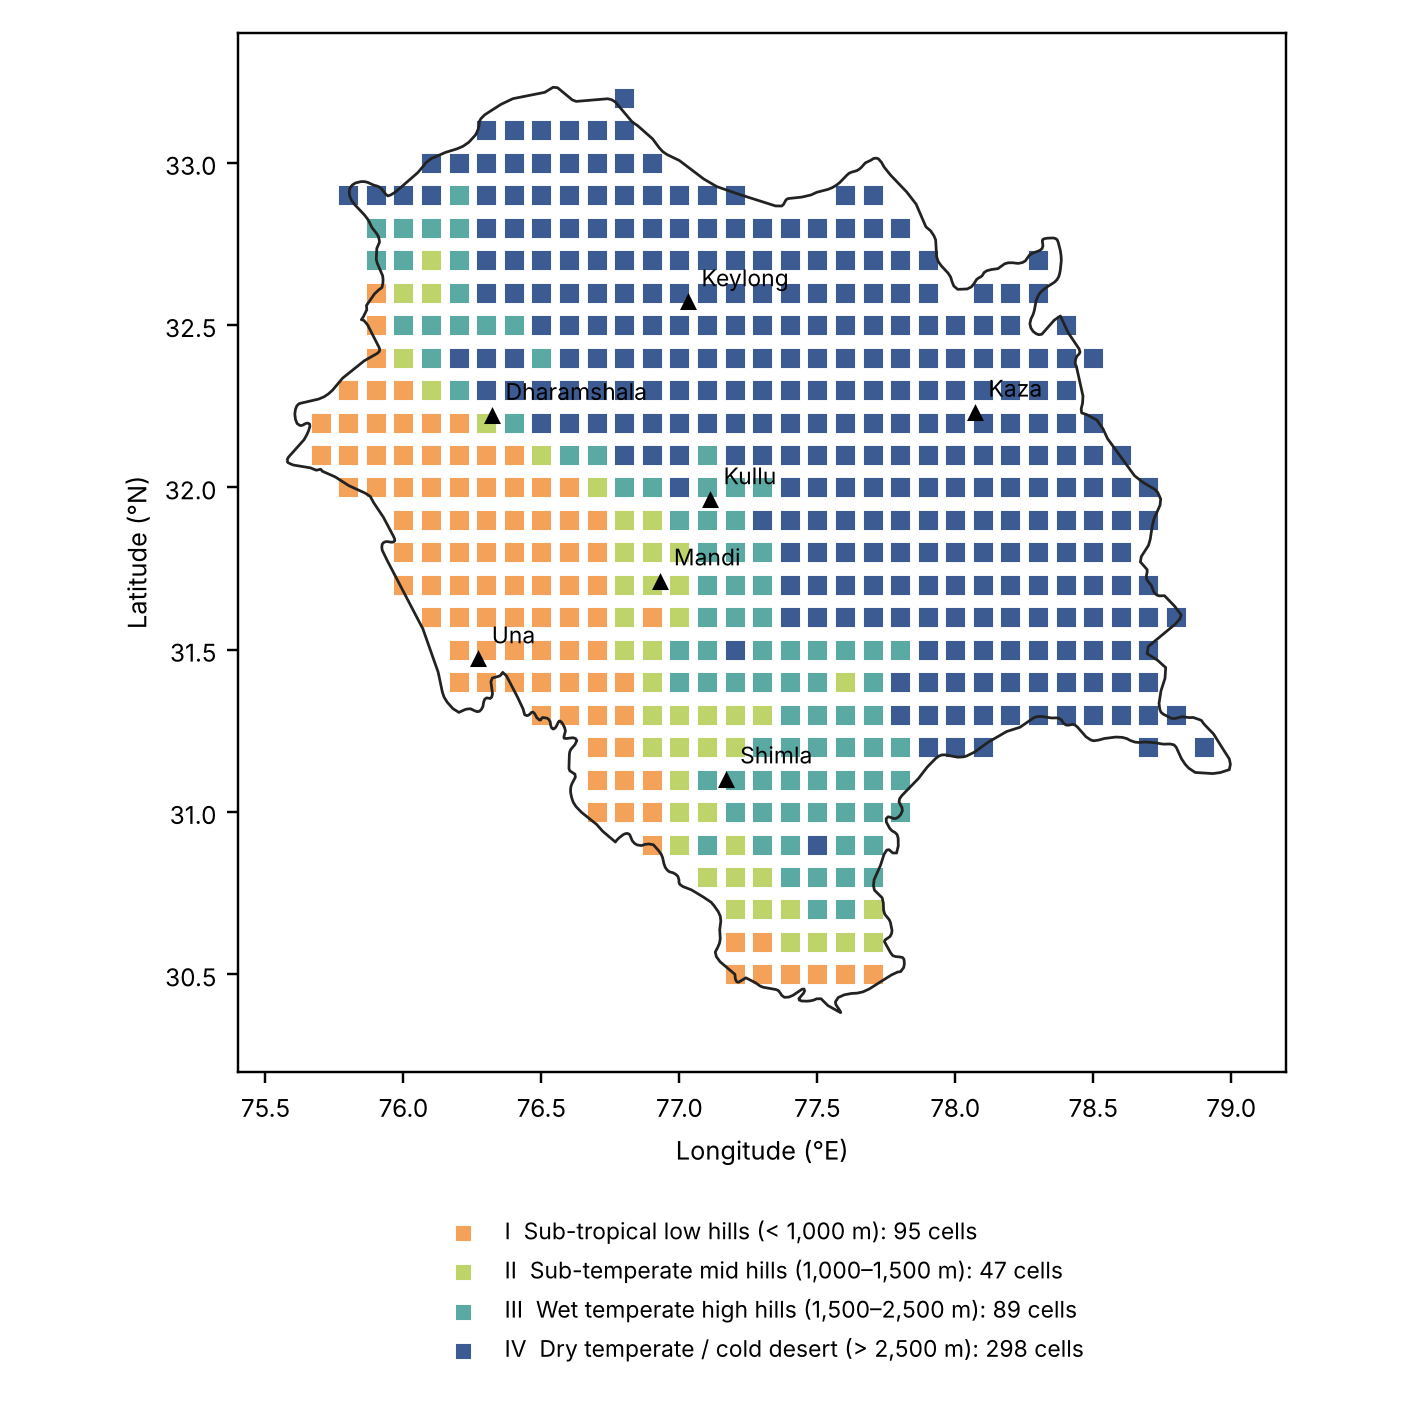
\includegraphics[width=0.66\textwidth]{fig_hp_zones.png}
\caption{The 529 grid cells of Himachal Pradesh coloured by elevation band (mean SRTM height of the cell). Triangles
mark towns for orientation.}
\label{fig:hpzones}
\end{figure}

\begin{itemize}
\item \textbf{Low hills (Una, Kangra valley, Bilaspur).} Hot pre-monsoon months with temperatures near those of the
Punjab plains, and a wet monsoon. Heatwaves from the plains reach here.
\item \textbf{Mid and high hills (Mandi, Shimla, Kullu).} Mild summers and cold winters with snow at higher places;
the heaviest monsoon rain falls on the outer ranges such as the Dhauladhar near Dharamshala.
\item \textbf{Cold desert (Lahaul--Spiti, upper Kinnaur).} Behind the Pir Panjal and Great Himalayan ranges, in their
rain shadow: little monsoon rain, snow mainly from western disturbances, very cold winters.
\end{itemize}

\textbf{Why this matters for the project.}
\begin{itemize}
\item The same temperature is ordinary in Una and extreme in Kaza, so a single national rule cannot describe extremes
everywhere. IMD itself uses different heatwave rules for plains (at least 40\,$^\circ$C) and hilly regions (at least
30\,$^\circ$C), together with a departure of 4.5\,$^\circ$C or more from normal. This project goes
one step further and uses the 99th percentile of each cell in each season (Chapter~\ref{ch:extreme}).
\item Seasons behave differently: pre-monsoon extremes are dry heat; monsoon extremes come in breaks of the monsoon;
winter extremes are warm spells between western disturbances. That is why thresholds and the EVT fit are computed per
season.
\item The factors above are what the predictors measure: elevation and slope (altitude and relief), soil moisture and
recent rain (land-surface dryness), humidity and dewpoint (monsoon moisture), surface pressure and its change
(passing disturbances) and solar radiation (clear skies).
\end{itemize}


\begin{sayit}
``India has four IMD rainfall regions; Himachal Pradesh is in Northwest India. Its weather is shaped by altitude, the
Himalaya, the monsoon and western disturbances. Because the state goes from 300\,m to over 6,000\,m, the same
temperature can be normal in Una and extreme in Kaza, so I define extremes per cell and per season.''
\end{sayit}
